% 注意事项:编译两次,以确保目录、页码完整显示

\def\allfiles{}

\documentclass[14pt,a4paper,UTF8,twoside]{article}

% Formatting Packages ——————————————————————————————————————
\usepackage{multicol}
\usepackage{multirow}
\usepackage{enumitem}
\usepackage{indentfirst}
\usepackage[toc]{multitoc}

% Math & Physics Packages ————————————————————————————
\usepackage{amsmath, amsthm, amsfonts, amssymb}
\usepackage{setspace}
\usepackage{physics}
\usepackage{cancel}
\usepackage{nicefrac}
\usepackage{unicode-math} % 允许数学公式使用特定字体

% Image-related Packages —————————————————————————————
\usepackage{float} % 浮动体环境
\usepackage{subcaption} % 子图包
\usepackage{graphics, graphicx}
\usepackage{tikz, tikz-qtree}
\usetikzlibrary{arrows.meta}
\usepackage{pgfplots}
\pgfplotsset{compat=1.18}
\usepackage{xcolor}
\usepackage{fourier-orns}
\usepackage{lipsum}

% Colour Palette ——————————————————————————————————————
\definecolor{merah}{HTML}{F4564E}
\definecolor{merahtua}{HTML}{89313E}
\definecolor{biru}{HTML}{60BBE5}
\definecolor{birutua}{HTML}{412F66}
\definecolor{hijau}{HTML}{59CC78}
\definecolor{hijautua}{HTML}{366D5B}
\definecolor{kuning}{HTML}{FFD56B}
\definecolor{jingga}{HTML}{FBA15F}
\definecolor{ungu}{HTML}{8C5FBF}
\definecolor{lavender}{HTML}{CBA5E8}
\definecolor{merjamb}{HTML}{FFB6E0}
\definecolor{mygray}{HTML}{E6E6E6}
\definecolor{mygreen}{rgb}{0,0.6,0}
\definecolor{mymauve}{rgb}{0.58,0,0.82}

% Theorems ————————————————————————————————————————————
\usepackage{tcolorbox}
\usepackage{changepage}
\tcbuselibrary{skins,breakable,theorems}

\newcounter{hitung}
\setcounter{hitung}{\thesection}

\makeatletter
	% Proof 证明如下
	\def\tcb@theo@widetitle#1#2#3{\hbox to \textwidth{\textsc{\large#1}\normalsize\space#3\hfil(#2)}}
	\tcbset{
		theorem style/theorem wide name and number/.code={ \let\tcb@theo@title=\tcb@theo@widetitle},
		proofbox/.style={skin=enhancedmiddle,breakable,parbox=false,boxrule=0mm,
			check odd page, toggle left and right, colframe=black!20!white!92!hijau,
			leftrule=8pt, rightrule=0mm, boxsep=0mm,arc=0mm, outer arc=0mm,
			left=3mm,right=3mm,top=0mm,bottom=0mm, toptitle=0mm,
			bottomtitle=0mm,colback=gray!3!white!98!biru, before skip=8pt, after skip=8pt,
			before={\par\vskip-2pt},after={\par\smallbreak},
		},
	}
	\newtcolorbox{ProofBox}{proofbox}
	\makeatother
	
	\let\realproof\proof
	\let\realendproof\endproof
	\renewenvironment{proof}[1][Prove:]{\ProofBox\strut\textsc{#1}\space}{\endProofBox}
        \AtEndEnvironment{proof}{\null\hfill$\blacksquare$}
        % Definition 定义环境
	\newtcbtheorem[use counter=hitung, number within=section]{dfn}{定义}
	{theorem style=theorem wide name and number,breakable,enhanced,arc=3.5mm,outer arc=3.5mm,
		boxrule=0pt,toprule=1pt,leftrule=0pt,bottomrule=1pt, rightrule=0pt,left=0.2cm,right=0.2cm,
		titlerule=0.5em,toptitle=0.1cm,bottomtitle=-0.1cm,top=0.2cm,
		colframe=white!10!biru,
		colback=white!90!biru,
		coltitle=white,
		shadow={1.3mm}{-1.3mm}{0mm}{gray!50!white}, % 添加阴影
        coltext=birutua!60!gray, title style={white!10!biru}, rbefoe skip=8pt, after skip=8pt,
		fonttitle=\bfseries,fontupper=\normalsize}{dfn}

	% 答题卡
	\newtcbtheorem[use counter=hitung, number within=section]{ans}{解答}
	{theorem style=theorem wide name and number,breakable,enhanced,arc=3.5mm,outer arc=3.5mm,
		boxrule=0pt,toprule=1pt,leftrule=0pt,bottomrule=1pt, rightrule=0pt,left=0.2cm,right=0.2cm,
		titlerule=0.5em,toptitle=0.1cm,bottomtitle=-0.1cm,top=0.2cm,
		colframe=white!10!biru,
		colback=white!90!biru,
		coltitle=white,
		shadow={1.3mm}{-1.3mm}{0mm}{gray!50!white}, % 添加阴影
        coltext=birutua!60!gray, title style={white!10!biru}, before skip=8pt, after skip=8pt,
		fonttitle=\bfseries,fontupper=\normalsize}{ans}

	% Axiom
	\newtcbtheorem[use counter=hitung, number within=section]{axm}{公理}
	{theorem style=theorem wide name and number,breakable,enhanced,arc=3.5mm,outer arc=3.5mm,
		boxrule=0pt,toprule=1pt,leftrule=0pt,bottomrule=1pt, rightrule=0pt,left=0.2cm,right=0.2cm,
		titlerule=0.5em,toptitle=0.1cm,bottomtitle=-0.1cm,top=0.2cm,
		colframe=white!10!biru,colback=white!90!biru,coltitle=white,
		shadow={1.3mm}{-1.3mm}{0mm}{gray!50!white!90}, % 添加阴影
        coltext=birutua!60!gray,title style={white!10!biru},before skip=8pt, after skip=8pt,
		fonttitle=\bfseries,fontupper=\normalsize}{axm}
 
	% Theorem
	\newtcbtheorem[use counter=hitung, number within=section]{thm}{定理}
	{theorem style=theorem wide name and number,breakable,enhanced,arc=3.5mm,outer arc=3.5mm,
		boxrule=0pt,toprule=1pt,leftrule=0pt,bottomrule=1pt, rightrule=0pt,left=0.2cm,right=0.2cm,
		titlerule=0.5em,toptitle=0.1cm,bottomtitle=-0.1cm,top=0.2cm,
		colframe=white!10!merah,colback=white!75!pink,coltitle=white, coltext=merahtua!80!merah,
		shadow={1.3mm}{-1.3mm}{0mm}{gray!50!white!90}, % 添加阴影
		title style={white!10!merah}, before skip=8pt, after skip=8pt,
		fonttitle=\bfseries,fontupper=\normalsize}{thm}
	
	% Proposition
	\newtcbtheorem[use counter=hitung, number within=section]{prp}{命题}
	{theorem style=theorem wide name and number,breakable,enhanced,arc=3.5mm,outer arc=3.5mm,
		boxrule=0pt,toprule=1pt,leftrule=0pt,bottomrule=1pt, rightrule=0pt,left=0.2cm,right=0.2cm,
		titlerule=0.5em,toptitle=0.1cm,bottomtitle=-0.1cm,top=0.2cm,
		colframe=white!10!hijau,colback=white!90!hijau,coltitle=white, coltext=hijautua!80!brown,
		shadow={1.3mm}{-1.3mm}{0mm}{gray!50!white}, % 添加阴影
		title style={white!10!hijau}, before skip=8pt, after skip=8pt,
		fonttitle=\bfseries,fontupper=\normalsize}{prp}


	% Example
	\newtcolorbox[use counter=hitung, number within=section]{cth}[1][]{breakable,
		colframe=white!10!jingga, coltitle=white!90!jingga, colback=white!85!jingga, coltext=black!10!brown!50!jingga, colbacktitle=white!10!jingga, enhanced, fonttitle=\bfseries,fontupper=\normalsize, attach boxed title to top left={yshift=-2mm}, before skip=8pt, after skip=8pt,
		title=Contoh~\thetcbcounter \ \ #1}

	% Catatan/Note
	\newtcolorbox{ctt}[1][]{enhanced, 
		left=4.1mm, borderline west={8pt}{0pt}{white!10!kuning}, 
		before skip=6pt, after skip=6pt, 
		colback=white!85!kuning, colframe= white!85!kuning, coltitle=orange!60!kuning!25!brown, coltext=orange!60!kuning!25!brown,
		fonttitle=\bfseries,fontupper=\normalsize, before skip=8pt, after skip=8pt,
		title=\underline{Catatan}  #1}
	
	% Komentar/Remark
	\newtcolorbox{rmr}[1][]{
		,arc=0mm,outer arc=0mm,
		boxrule=0pt,toprule=1pt,leftrule=0pt,bottomrule=5pt, rightrule=0pt,left=0.2cm,right=0.2cm,
		titlerule=0.5em,toptitle=0.1cm,bottomtitle=-0.1cm,top=0.2cm,
		colframe=white!10!kuning,colback=white!85!kuning,coltitle=white, coltext=orange!60!kuning,
		fonttitle=\bfseries,fontupper=\normalsize, before skip=8pt, after skip=8pt,
		title=Komentar  #1}

\usepackage{booktabs} % 表格库
\usepackage{titlesec} % 标题库
\usepackage{fancyhdr} % 页眉页脚库
\usepackage[sorting=none]{biblatex}
\usepackage{array}
\addbibresource{references.bib} % 指定你的.bib文件名称

\date{} % 留空,以让编译时去除日期

%———————————————注意事项—————————————————%

% 1、如果编译显示失败,但没有错误信息,就是 filename.pdf 正在被占用
% 2、在文件夹中的终端使用 Windows > xelatex filename.tex 也可编译

%—————————————华东师范大学———————————————%

% 论文制作时须加页眉,页眉从中文摘要开始至论文末
% 偶数页码内容为:华东师范大学硕士学位论文,奇数页码内容为学位论文题目

%————————定义 \section 的标题样式————————%

% 注意:\chapter 等命令,内部使用的是 \thispagestyle{plain} 的排版格式
% 若需要自己加上页眉,实际是在用 \thispagestyle{fancy} 的排版格式
% 加上下面这一段指令,就能够让 \section 也使用 fancy 的排版格式
% 本质就是让目录、第一页也能够显示页眉、页脚

\fancypagestyle{plain}{
  \pagestyle{fancy}
}

\title{华东师范大学软件学院课程作业} % 模板
\titleformat{\section}
    {\normalfont\bfseries\Large} % 字体大小、字体系列(\bfseries 为加粗)
    {\thesection}{1em}{}

% ———————————设置章节的中文格式———————————%
\renewcommand\thesection{\chinese{section} \hspace{0pt}}
\renewcommand\thesubsection{\arabic{subsection} \hspace{0pt}}
% \renewcommand\thesubsubsection{\alph{subsubsection} \hspace{0pt}} % 字母编号
% \hspace{0pt} 是为了确保在章节编号和章节题目之间不要有空格,使得排版更为美观
    
%—————————————页面基础设置———————————————%

\usepackage{geometry}
\geometry{left=10mm, right=10mm, top=20mm, bottom=20mm}

%————————————设置页眉、页脚——————————————%

\pagestyle{fancy} % 设置 plain style 的属性

% 设置页眉

\fancyhead[RE]{\footnotesize \leftmark} % Right Even 偶数页右侧显示章名 \leftmark 最高级别章名
\fancyhead[LO]{\footnotesize \rightmark} % Left Odd 奇数页左侧显示节名 \rightmark 第二级别节名
\fancyhead[C]{华东师范大学软件学院课程作业} % Center 居中显示
\fancyhead[LE,RO]{~\thepage~} % 在偶数页的左侧,奇数页的右侧显示页码
\renewcommand{\headrulewidth}{1.2pt} % 页眉与正文之间的水平线粗细

% 设置页脚:在每页的右下脚以斜体显示书名

\fancyfoot[RO,RE]{\it Lab Report By \LaTeX} % 使用意大利斜体显示
\renewcommand{\footrulewidth}{0.5pt} % 页脚水平线宽度

%——————设置页码:在底部居中显示页码———————%

\usepackage{lastpage} % 页码数库
\pagestyle{fancy}
\fancyfoot[C]{\kaishu 第 \thepage 页 \ 共 \pageref{LastPage} 页} % LastPage 需要二次编译以获取总页数

%——————————————代码块设置———————————————%

\usepackage{listings} % 代码块包
\lstset {
    backgroundcolor=\color{white},   % choose the background color; you must add \usepackage{color} or \usepackage{xcolor}
    basicstyle=\footnotesize,        % the size of the fonts that are used for the code
    breakatwhitespace=false,         % sets if automatic breaks should only happen at whitespace
    breaklines=true,                 % sets automatic line breaking
    captionpos=bl,                   % sets the caption-position to bottom
    commentstyle=\color{mygreen},    % comment style
    deletekeywords={...},            % if you want to delete keywords from the given language
    escapeinside={\%*}{*},           % if you want to add LaTeX within your code
    extendedchars=true,              % lets you use non-ASCII characters; for 8-bits encodings only, does not work with UTF-8
    frame=single,                    % adds a frame around the code
    keepspaces=true,                 % keeps spaces in text, useful for keeping indentation of code (possibly needs columns=flexible)
    keywordstyle=\color{blue},       % keyword style
    % language=Python,               % the language of the code
    morekeywords={*,...},            % if you want to add more keywords to the set
    numbers=left,                    % where to put the line-numbers; possible values are (none, left, right)
    numbersep=5pt,                   % how far the line-numbers are from the code
    numberstyle=\tiny\color{mygray}, % the style that is used for the line-numbers
    rulecolor=\color{black},         % if not set, the frame-color may be changed on line-breaks within not-black text (e.g. comments (green here))
    showspaces=false,                % show spaces everywhere adding particular underscores; it overrides 'showstringspaces'
    showstringspaces=false,          % underline spaces within strings only
    showtabs=false,                  % show tabs within strings adding particular underscores
    stepnumber=1,                    % the step between two line-numbers. If it's 1, each line will be numbered
    stringstyle=\color{orange},      % string literal style
    tabsize=2,                       % sets default tabsize to 2 spaces
    % title=Python Code              % show the filename of files included with \lstinputlisting; also try caption instead of title
}

% 注释掉的部分用于后续插入代码,参数可调整,格式如下:

% 1、直接插入
% \begin{lstlisting}[language = ? , title = { ? } ]
%       Your code here.
% \end{lstlisting}

% 2、文件插入
% \lstinputlisting[language = C , title = ?.c] {filename.c}

%———————————————字体设置————————————————%

\usepackage{fontspec} % 允许设置字体
\usepackage[utf8]{inputenc}
\usepackage{ctex}
\linespread{1.2}
% \setCJKmainfont{SimSun} % 设置正文罗马族的 CJK 字体

%———————————————超链接设置——————————————%

\usepackage[hidelinks]{hyperref}
\hypersetup{
    pdfstartview=FitH, % 设置PDF文档打开时的初始视图为页面宽度适应窗口宽度(即页面水平适应)
    CJKbookmarks=true, % 用对CJK(中文、日文、韩文)字符的书签支持,确保这些字符在书签中正确显示
    bookmarksnumbered=true, % 书签带有章节编号。这对有章节编号的文档很有用
    bookmarksopen=true, % 文档打开时,书签树是展开的,方便查看所有书签
    colorlinks, % 启用彩色链接。这样,链接在PDF中会显示为彩色,而不是默认的方框
    pdfborder=001, % 设置PDF文档中链接的边框样式。001 表示链接周围没有边框,仅在单击时显示一个矩形
    linkcolor=blue, % 设置文档内部链接(如目录中的章节链接)的颜色为蓝色
    anchorcolor=blue, % 设置锚点链接(即目标在同一文档内的链接)的颜色为蓝色
    citecolor=blue, % 设置引用(如文献引用)的颜色为蓝色
}

%——————————————导言区结束,进入正文部分———————————————%

\begin{document}

\maketitle

\begin{center} % \extracolsep{\fill} 拉伸到页面最大宽度前,保证居中显示

  \begin{tabular*}{\textwidth}{@{\extracolsep{\fill}} l  l  l }
    \hline
    课程名称:软件质量分析 &  年级:2023级本科  &  姓名:张梓卫 \\
    作业主题:游戏服务器系统的可信度量 & 学号:10235101526 & 作业日期:2024/12/04 \\
    指导老师:陈仪香 & 组号: \\
    \hline
  \end{tabular*}

\end{center}

\tableofcontents % 目录也需要二次编译

\section{基于组件的软件可信性度量模型}

\subsection{权重向量的计算}

首先需要计算 EV、LLSM、CSM,我们可以拿 Homework 6 的算法直接使用:

\begin{lstlisting} [language = Python, title = Homework 6]
import numpy as np

A = np.array([
    [1, 2, 1/2, 2, 1/4],
    [1/2, 1, 2, 3, 1/2],
    [2, 1/2, 1, 1, 1/2],
    [1/2, 1/3, 1, 1, 1/2],
    [4, 2, 2, 2, 1]
])

def calculate_ev_weights(matrix):
    eigenvalues, eigenvectors = np.linalg.eig(matrix)  # 返回值为元组,第一个元素为特征值,第二个元素为特征向量
    max_index = np.argmax(eigenvalues)  # 取最大特征值对应的特征向量
    weights = eigenvectors[:, max_index].real
    # 归一化
    return weights / np.sum(weights)

def calculate_llsm_weights(matrix):
    # 分子 = 每行的乘积 × 开维度数次方
    numerator = np.prod(matrix, axis=1) ** (1 / matrix.shape[0])
    # 分母 = 每行的分子相加
    denominator =  np.sum(numerator)
    # 归一化
    return numerator / denominator

def calculate_csm_weights(matrix: np.array, epsilon: float, max_iterations: int) -> np.ndarray:
    '''计算 CSM,传入: matrix, precision, maximum iterations'''
    n = matrix.shape[0]
    # 初始化初始解
    W = np.ones(n) / n

    for k in range(max_iterations):
        e = np.zeros(n)
        for i in range(n):
            e[i] = np.sum([(1 + matrix[j, i] ** 2) * (W[i] / W[j]) - (1 + matrix[i, j] ** 2) * (W[j] / W[i])
                           for j in range(n) if j != i])

        max_e = np.max(np.abs(e))
        if max_e <= epsilon: # 若精度已到达,那么停止迭代
            print(f"CSM 算法在迭代次数为 {k} 次时收敛")
            break

        m = np.argmax(np.abs(e)) # 查找最大无差的索引

        # 计算 T(k)
        up = np.sum([(1 + matrix[m, j] ** 2) * (W[j] / W[m]) for j in range(n) if j != m])
        bottom = np.sum([(1 + matrix[j, m] ** 2) * (W[m] / W[j]) for j in range(n) if j != m])
        T = np.sqrt(up / bottom)

        # 更新矩阵向量,归一化
        X = W.copy()
        X[m] *= T
        W = X / np.sum(X)

    return W

def calculate_td(matrix: np.array, weight_vector: np.ndarray) -> float:
    n = len(weight_vector)
    td = 0.0
    for i in range(n):
        for j in range(n):
            td += abs(matrix[i, j] - (weight_vector[i] / weight_vector[j]))
    return td

weights_ev = calculate_ev_weights(A)
print("判断矩阵:\n", A)
print("权重向量 EV:", weights_ev)

weights_llsm = calculate_llsm_weights(A)
print("权重向量 LLSM:", weights_llsm)

weights_csm = calculate_csm_weights(A, 1e-10, 1000)
print("CSM 权重向量:", weights_csm)

TD_EV = calculate_td(A, weights_ev)
TD_LLSM = calculate_td(A, weights_llsm)
TD_CSM = calculate_td(A, weights_csm)

print("TD EV:", TD_EV)
print("TD LLSM:", TD_LLSM)
print("TD CSM:", TD_CSM)

td_values = {"EV": TD_EV, "LLSM": TD_LLSM, "CSM": TD_CSM}
min_method = min(td_values, key=td_values.get)
print(f"最小的 TD 值为 {td_values[min_method]},选 {min_method} 计算的权重向量为可信属性的权重向量。")
\end{lstlisting}

将关键组件的矩阵 A 输入到代码中,输出结果为:

\begin{figure} [H]
    \centering
    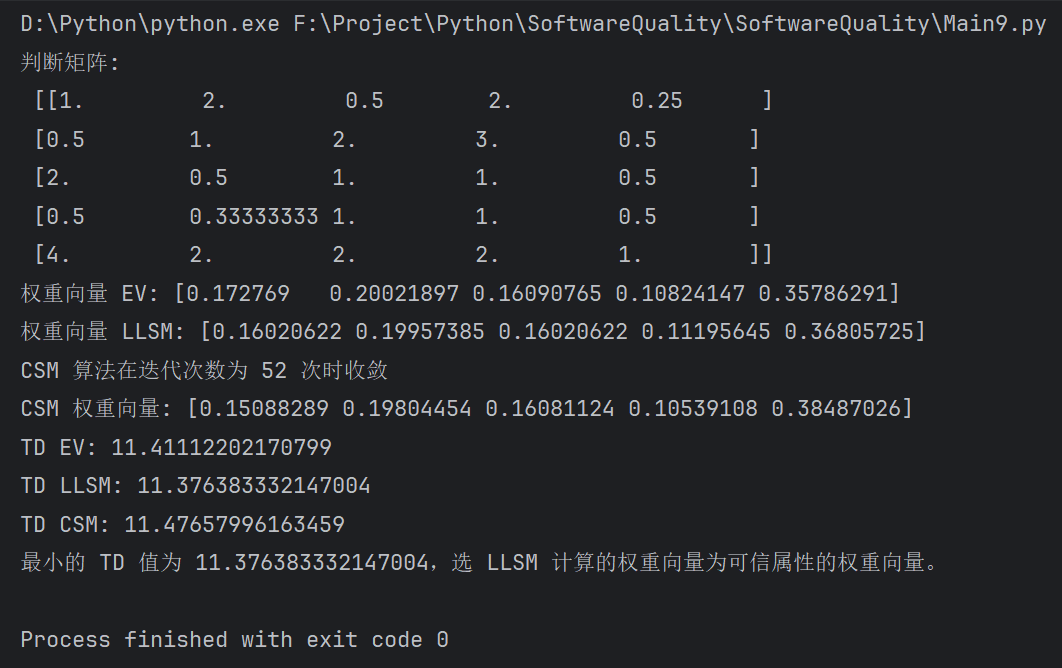
\includegraphics[width = 0.5\textwidth]{img9/weights.png}
    \caption{权重向量}
    \label{fig:first}
\end{figure}

整理如下:

\begin{ans}{关键组件}{关键组件}
    \textbf{正互反判断矩阵}:
    \[
    A = 
    \begin{bmatrix}
    1 & 2 & \frac{1}{2} & 2 & \frac{1}{4} \\
    \frac{1}{2} & 1 & 2 & 3 & \frac{1}{2} \\
    2 & \frac{1}{2} & 1 & 1 & \frac{1}{2} \\
    \frac{1}{2} & \frac{1}{3} & 1 & 1 & \frac{1}{2} \\
    4 & 2 & 2 & 2 & 1 \\
    \end{bmatrix}
    \]
  \end{ans}
    
  \bigskip
    
  \begin{table}[H]
    \centering
    \begin{tabular}{c|c}
    \hline
    方法 & 权重向量 \\ 
    \hline
    EV   & (0.1728, 0.2002, 0.1609, 0.1082, 0.3579) \\ 
    LLSM & (0.1602, 0.1996, 0.1602, 0.1120, 0.3681) \\ 
    CSM  & (0.1509, 0.1980, 0.1608, 0.1054, 0.3849) \\ 
    \hline
    \end{tabular}
  \end{table}
  
\begin{center}
  三个权重向量的值分别为 $ TD^{EV} = 11.4111, TD^{LLSM} = 11.3764, TD^{CSM} = 11.4766 $。
  
  最小的 TD 值为 $ 11.3764 $,选 LLSM 计算的权重向量为可信属性的权重向量。
\end{center}

\begin{table}[H]
    \centering
    \caption{关键组件正互反判断矩阵及权重}
    \label{tab:critical_weights}
    \begin{tabular}{|c|c|c|c|c|c|c|}
    \hline
    \textbf{组件名} & \textbf{CP1} & \textbf{CP2} & \textbf{CP3} & \textbf{CP4} & \textbf{CP5} & \textbf{属性权重} \\ \hline
    \textbf{CP1}   & 1            & 2            & 1/2          & 2            & 1/4          & 0.1602           \\ \hline
    \textbf{CP2}   & 1/2          & 1            & 2            & 3            & 1/2          & 0.1996           \\ \hline
    \textbf{CP3}   & 2            & 1/2          & 1            & 1            & 1/2          & 0.1602           \\ \hline
    \textbf{CP4}   & 1/2          & 1/3          & 1            & 1            & 1/2          & 0.1120           \\ \hline
    \textbf{CP5}   & 4            & 2            & 2            & 2            & 1            & 0.3681           \\ \hline
    \end{tabular}
\end{table}

同理,非关键组件代入矩阵 A,得到的结果如下:

\begin{figure} [H]
    \centering
    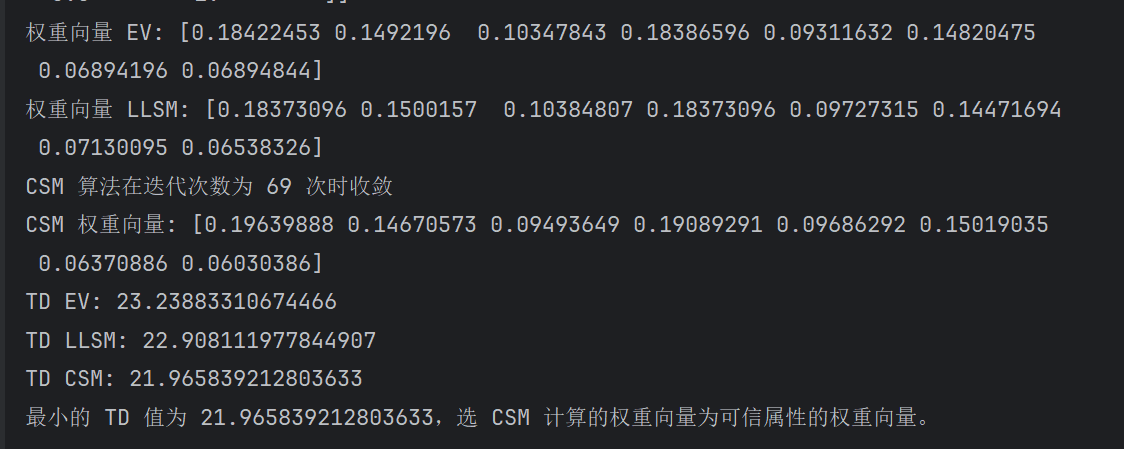
\includegraphics[width = 0.5\textwidth]{img9/weights2.png}
    \caption{权重向量}
    \label{fig:first}
\end{figure}

\begin{ans}{非关键组件}{非关键组件}
    \textbf{正互反判断矩阵}:
    \[
    A = 
    \begin{bmatrix}
    1 & 3 & 2 & \frac{1}{2} & 2 & 1 & 3 & 3 \\
    \frac{1}{3} & 1 & 2 & 1 & 2 & 2 & 2 & 2 \\
    \frac{1}{2} & \frac{1}{2} & 1 & \frac{1}{2} & 1 & \frac{1}{2} & 3 & 3 \\
    2 & 1 & 2 & 1 & 3 & \frac{1}{2} & 3 & 3 \\
    \frac{1}{2} & \frac{1}{2} & 1 & \frac{1}{3} & 1 & 1 & 2 & 2 \\
    1 & \frac{1}{2} & 2 & 2 & 1 & 1 & 2 & 2 \\
    \frac{1}{3} & \frac{1}{2} & 1 & \frac{1}{3} & \frac{1}{2} & \frac{1}{2} & 1 & 2 \\
    \frac{1}{3} & \frac{1}{2} & 2 & \frac{1}{3} & \frac{1}{2} & \frac{1}{2} & \frac{1}{2} & 1 \\
    \end{bmatrix}
    \]
  \end{ans}
    
  \bigskip
    
  \begin{table}[H]
    \centering
    \begin{tabular}{c|c}
    \hline
    方法 & 权重向量 \\ 
    \hline
    EV   & (0.1842, 0.1492, 0.1035, 0.1839, 0.0931, 0.1482, 0.0689, 0.0689) \\ 
    LLSM & (0.1837, 0.1500, 0.1038, 0.1837, 0.0973, 0.1447, 0.0713, 0.0654) \\ 
    CSM  & (0.1964, 0.1467, 0.0949, 0.1909, 0.0969, 0.1502, 0.0637, 0.0603) \\ 
    \hline
    \end{tabular}
  \end{table}
  
  \begin{center}
  三个权重向量的值分别为 $ TD^{EV} = 23.2388, TD^{LLSM} = 22.9081, TD^{CSM} = 21.9658 $。
  
  最小的 TD 值为 $ 21.9658 $,选 CSM 计算的权重向量为可信属性的权重向量。
  \end{center}

  \begin{table}[H]
    \centering
    \caption{非关键组件正互反判断矩阵及权重}
    \label{tab:non_critical_weights}
    \begin{tabular}{|c|c|c|c|c|c|c|c|c|c|}
    \hline
    \textbf{组件名} & \textbf{CP6} & \textbf{CP7} & \textbf{CP8} & \textbf{CP9} & \textbf{CP10} & \textbf{CP11} & \textbf{CP12} & \textbf{CP13} & \textbf{属性权重} \\ \hline
    \textbf{CP6}   & 1            & 3            & 2            & 1/2          & 2             & 1             & 3             & 3             & 0.1964           \\ \hline
    \textbf{CP7}   & 1/3          & 1            & 2            & 1            & 2             & 2             & 2             & 2             & 0.1467           \\ \hline
    \textbf{CP8}   & 1/2          & 1/2          & 1            & 1/2          & 1             & 1/2           & 3             & 3             & 0.0949           \\ \hline
    \textbf{CP9}   & 2            & 1            & 2            & 1            & 3             & 1/2           & 3             & 3             & 0.1909           \\ \hline
    \textbf{CP10}  & 1/2          & 1/2          & 1            & 1/3          & 1             & 1             & 2             & 2             & 0.0969           \\ \hline
    \textbf{CP11}  & 1            & 1/2          & 2            & 2            & 1             & 1             & 2             & 2             & 0.1502           \\ \hline
    \textbf{CP12}  & 1/3          & 1/2          & 1            & 1/3          & 1/2           & 1/2           & 1             & 2             & 0.0637           \\ \hline
    \textbf{CP13}  & 1/3          & 1/2          & 2            & 1/3          & 1/2           & 1/2           & 1/2           & 1             & 0.0603           \\ \hline
    \end{tabular}
\end{table}


\subsection{计算$T_s$的值}

先写出整体最重要的函数部分,如下所示:

\begin{lstlisting} [language = Python, title = Ts]
    def calculate_system_trustworthiness(
        Critical_Confidence_value, Non_Critical_Confidence_value,
        alpha, beta, FC, NFC
):
    """
    计算系统可信度值 T_S

    参数:
    - Critical_Confidence_value: 关键组件的可信值数组 (numpy array)
    - Non_Critical_Confidence_value: 非关键组件的可信值数组 (numpy array)
    - alpha: 关键组件权重系数
    - beta: 非关键组件权重系数
    - FC: 关键组件权重向量 (numpy array)
    - NFC: 非关键组件权重向量 (numpy array)

    返回:
    - 系统可信度值 T_S
    """
    critical_product = np.prod(
        np.power(Critical_Confidence_value, FC)
    )
    print(f"关键属性乘积: {critical_product}")

    non_critical_product = np.prod(
        np.power(Non_Critical_Confidence_value, NFC)
    )
    print(f"非关键属性乘积: {non_critical_product}")

    T_S = alpha * critical_product + beta * non_critical_product

    return T_S
\end{lstlisting}

接下来,我们可以计算关键组件的可信值数组和非关键组件的可信值数组,并输入到函数中:

\begin{lstlisting} [language = Python, title = Ts]
    alpha = 0.7
    beta = 0.3
    print(f"此时的 Alpha 值为 {alpha}, Beta 值为 {beta}")
    
    T_S = calculate_system_trustworthiness(
        Critical_Confidence_value, Non_Critical_Confidence_value,
        alpha, beta, final_critical_weights, final_non_critical_weights
    )
    
    print(f"Ts的值为:{T_S}")
\end{lstlisting}

调整 $\alpha$ 和 $\beta$ 的值,可以得到不同的 $T_s$ 值。

示例输出如下:

\begin{figure}[H]
    \centering
    \begin{subfigure}{0.55\textwidth}
        \centering
        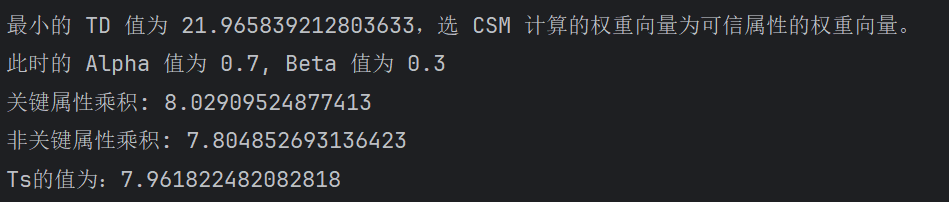
\includegraphics[width=\textwidth]{img9/Ts.png}
        \label{fig:Ts}
    \end{subfigure}
    
    \vspace{0.25cm} % 调整间距
    
    \begin{subfigure}{0.55\textwidth}
        \centering
        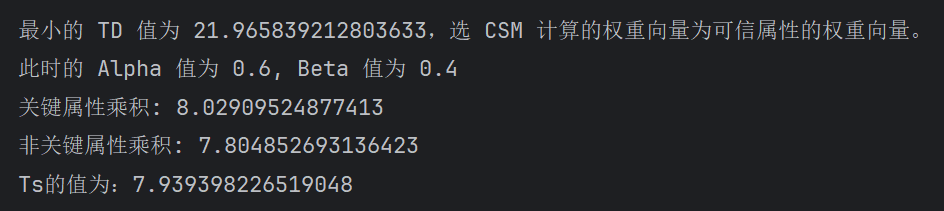
\includegraphics[width=\textwidth]{img9/Ts2.png}
        \label{fig:Ts2}
    \end{subfigure}
    
    \vspace{0.25cm} % 调整间距
    
    \begin{subfigure}{0.55\textwidth}
        \centering
        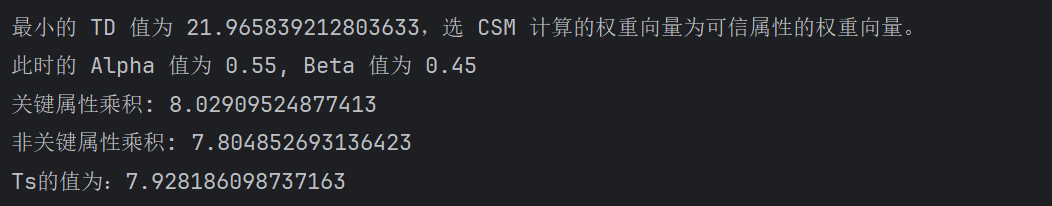
\includegraphics[width=\textwidth]{img9/Ts3.png}
        \label{fig:Ts3}
    \end{subfigure}
    
    \caption{不同 Ts 值的对比}
    \label{fig:Ts_combined}
\end{figure}

最后,我们可以制作为 Ts 的表格,如下所示:

\begin{table}[H]
    \centering
    \begin{tabular}{|c|c|c|}
    \hline
    \textbf{Alpha} & \textbf{Beta} & \textbf{$T_s$ 值} \\ \hline
    0.70 & 0.30 & 7.9618 \\ \hline
    0.60 & 0.40 & 7.9394 \\ \hline
    0.55 & 0.45 & 7.9282 \\ \hline
    \end{tabular}
    \label{tab:alpha_beta_ts}
\end{table}

\subsection{可信等级}

根据表格中的评判标准,我们可以轻易看出

\begin{figure}[H]
    \centering
    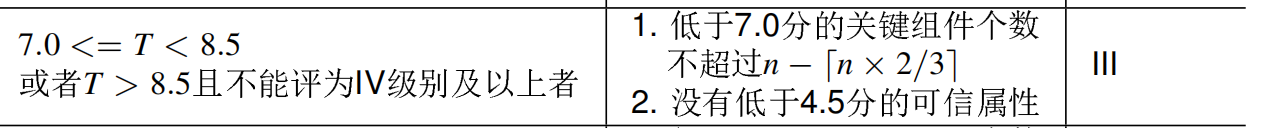
\includegraphics[width = 0.5\textwidth]{img9/direct.png}
    \caption{可信等级}
    \label{fig:trust_level}
\end{figure}

显然所有的关键属性都没有低于 7.0 分的,而 $T_s \ge 7$ 在不同的 $\alpha $ 和 $\beta $ 之下都成立。

故可信软件等级为 \textbf{III},当然,我们还可以编写代码来实现:

\begin{lstlisting} [language = Python, title = 可信等级代码]
    def classify_trust_level(T, scores):
    """
    分类可信等级
    :param: T: 系统可信度值
    :param: scores: 可信属性值数组
    :return: 可信等级
    """
    n = len(scores)
    threshold_2_3 = n - int(np.ceil(2 * n / 3))  # 计算 n - ⌈n × 2/3⌉

    # 统计低于某些阈值的属性个数
    low_9_5 = np.sum(scores < 9.5)
    low_8_5 = np.sum(scores < 8.5)
    low_7_0 = np.sum(scores < 7.0)
    low_4_5 = np.sum(scores < 4.5)

    if T >= 9.5:
        if low_9_5 <= threshold_2_3 and low_8_5 == 0:
            return "V"

    if 8.5 <= T < 9.5 or (T > 9.5):
        if low_8_5 <= threshold_2_3 and low_7_0 == 0:
            return "IV"

    if 7.0 <= T < 8.5 or (T > 8.5):
        if low_7_0 <= threshold_2_3 and low_4_5 == 0:
            return "III"

    if 4.5 <= T < 7.0 or (T > 7.0):
        if low_4_5 <= threshold_2_3:
            return "II"

    if T < 4.5 or (T > 4.5):
        return "I"
\end{lstlisting}

\section{附录}
\subsection{完整可执行代码}

\begin{lstlisting} [language = Python, title = 完整代码]
    from pprint import pprint

    import numpy as np
    
    # 作业
    Critical_Confidence_value = np.array([8.430, 8.530, 6.042, 9.094, 8.289])
    
    Non_Critical_Confidence_value = np.array([6.192, 8.020, 7.984, 8.713, 9.211, 7.777, 7.897, 8.075])
    
    Critical_A = np.array([
        [1, 2, 1/2, 2, 1/4],
        [1/2, 1, 2, 3, 1/2],
        [2, 1/2, 1, 1, 1/2],
        [1/2, 1/3, 1, 1, 1/2],
        [4, 2, 2, 2, 1]
    ])
    
    Non_Critical_A = np.array([
        [1, 3, 2, 1/2, 2, 1, 3, 3],
        [1/3, 1, 2, 1, 2, 2, 2, 2],
        [1/2, 1/2, 1, 1/2, 1, 1/2, 3, 3],
        [2, 1, 2, 1, 3, 1/2, 3, 3],
        [1/2, 1/2, 1, 1/3, 1, 1, 2, 2],
        [1, 1/2, 2, 2, 1, 1, 2, 2],
        [1/3, 1/2, 1, 1/3, 1/2, 1/2, 1, 2],
        [1/3, 1/2, 2, 1/3, 1/2, 1/2, 1/2, 1]
    ])
    
    # Test Data
    #
    # Critical_Confidence_value = np.array([9.536, 7.531, 9.167, 8.423])
    #
    # Non_Critical_Confidence_value = np.array([7.556, 7.858, 8.979, 7.708, 9.265])
    #
    # Critical_A = np.array([
    #     [1, 2, 1/2, 1/3],
    #     [1/2, 1, 1/2, 1/3],
    #     [2, 2, 1, 1/2],
    #     [3, 3, 2, 1]
    # ])
    #
    # Non_Critical_A = np.array([
    #     [1, 1/2, 1, 1/3, 1/2],
    #     [2, 1  , 2, 1/2, 1],
    #     [1, 1/2, 1, 1/2, 1],
    #     [3, 2  , 2, 1  , 2],
    #     [2, 1  , 1, 1/2, 1]
    # ])
    
    
    def classify_trust_level(T, scores):
        """
        分类可信等级
        :param: T: 系统可信度值
        :param: scores: 可信属性值数组
        :return: 可信等级
        """
        n = len(scores)
        threshold_2_3 = n - int(np.ceil(2 * n / 3))  # 计算 n - ⌈n × 2/3⌉
    
        # 统计低于某些阈值的属性个数
        low_9_5 = np.sum(scores < 9.5)
        low_8_5 = np.sum(scores < 8.5)
        low_7_0 = np.sum(scores < 7.0)
        low_4_5 = np.sum(scores < 4.5)
    
        if T >= 9.5:
            if low_9_5 <= threshold_2_3 and low_8_5 == 0:
                return "V"
    
        if 8.5 <= T < 9.5 or (T > 9.5):
            if low_8_5 <= threshold_2_3 and low_7_0 == 0:
                return "IV"
    
        if 7.0 <= T < 8.5 or (T > 8.5):
            if low_7_0 <= threshold_2_3 and low_4_5 == 0:
                return "III"
    
        if 4.5 <= T < 7.0 or (T > 7.0):
            if low_4_5 <= threshold_2_3:
                return "II"
    
        if T < 4.5 or (T > 4.5):
            return "I"
    
    
    def calculate_system_trustworthiness(
            Critical_Confidence_value, Non_Critical_Confidence_value,
            alpha, beta, FC, NFC
    ):
        """
        计算系统可信度值 T_S
    
        参数:
        - Critical_Confidence_value: 关键组件的可信值数组 (numpy array)
        - Non_Critical_Confidence_value: 非关键组件的可信值数组 (numpy array)
        - alpha: 关键组件权重系数
        - beta: 非关键组件权重系数
        - FC: 关键组件权重向量 (numpy array)
        - NFC: 非关键组件权重向量 (numpy array)
    
        返回:
        - 系统可信度值 T_S
        """
        critical_product = np.prod(
            np.power(Critical_Confidence_value, FC)
        )
        print(f"关键属性乘积: {critical_product}")
    
        non_critical_product = np.prod(
            np.power(Non_Critical_Confidence_value, NFC)
        )
        print(f"非关键属性乘积: {non_critical_product}")
    
        T_S = alpha * critical_product + beta * non_critical_product
    
        return T_S
    
    def calculate_ev_weights(matrix):
        eigenvalues, eigenvectors = np.linalg.eig(matrix)  # 返回值为元组,第一个元素为特征值,第二个元素为特征向量
        max_index = np.argmax(eigenvalues)  # 取最大特征值对应的特征向量
        weights = eigenvectors[:, max_index].real
        # 归一化
        return weights / np.sum(weights)
    
    def calculate_llsm_weights(matrix):
        # 分子 = 每行的乘积 × 开维度数次方
        numerator = np.prod(matrix, axis=1) ** (1 / matrix.shape[0])
        # 分母 = 每行的分子相加
        denominator =  np.sum(numerator)
        # 归一化
        return numerator / denominator
    
    def calculate_csm_weights(matrix: np.array, epsilon: float, max_iterations: int) -> np.ndarray:
        '''计算 CSM,传入: matrix, precision, maximum iterations'''
        n = matrix.shape[0]
        # 初始化初始解
        W = np.ones(n) / n
    
        for k in range(max_iterations):
            e = np.zeros(n)
            for i in range(n):
                e[i] = np.sum([(1 + matrix[j, i] ** 2) * (W[i] / W[j]) - (1 + matrix[i, j] ** 2) * (W[j] / W[i])
                               for j in range(n) if j != i])
    
            max_e = np.max(np.abs(e))
            if max_e <= epsilon: # 若精度已到达,那么停止迭代
                print(f"CSM 算法在迭代次数为 {k} 次时收敛")
                break
    
            m = np.argmax(np.abs(e)) # 查找最大无差的索引
    
            # 计算 T(k)
            up = np.sum([(1 + matrix[m, j] ** 2) * (W[j] / W[m]) for j in range(n) if j != m])
            bottom = np.sum([(1 + matrix[j, m] ** 2) * (W[m] / W[j]) for j in range(n) if j != m])
            T = np.sqrt(up / bottom)
    
            # 更新矩阵向量,归一化
            X = W.copy()
            X[m] *= T
            W = X / np.sum(X)
    
        return W
    
    def calculate_td(matrix: np.array, weight_vector: np.ndarray) -> float:
        n = len(weight_vector)
        td = 0.0
        for i in range(n):
            for j in range(n):
                td += abs(matrix[i, j] - (weight_vector[i] / weight_vector[j]))
        return td
    
    
    print("——————————————————————")
    print("以下是关键组件的判断矩阵:")
    
    
    print("判断矩阵:")
    pprint(Critical_A)
    print("——————————————————————")
    
    weights_ev = calculate_ev_weights(Critical_A)
    print("权重向量 EV:", weights_ev)
    
    weights_llsm = calculate_llsm_weights(Critical_A)
    print("权重向量 LLSM:", weights_llsm)
    
    weights_csm = calculate_csm_weights(Critical_A, 1e-10, 1000)
    print("CSM 权重向量:", weights_csm)
    
    TD_EV = calculate_td(Critical_A, weights_ev)
    TD_LLSM = calculate_td(Critical_A, weights_llsm)
    TD_CSM = calculate_td(Critical_A, weights_csm)
    
    print("TD EV:", TD_EV)
    print("TD LLSM:", TD_LLSM)
    print("TD CSM:", TD_CSM)
    
    td_values = {"EV": TD_EV, "LLSM": TD_LLSM, "CSM": TD_CSM}
    min_method = min(td_values, key=td_values.get)
    print(f"最小的 TD 值为 {td_values[min_method]},选 {min_method} 计算的权重向量为可信属性的权重向量。")
    final_critical_weights = weights_ev if min_method == "EV" else weights_llsm if min_method == "LLSM" else weights_csm
    
    print("————————————————————————")
    print("以下是非关键组件的判断矩阵:")
    
    print("判断矩阵:")
    pprint(Non_Critical_A)
    print("——————————————————————")
    
    weights_ev = calculate_ev_weights(Non_Critical_A)
    print("权重向量 EV:", weights_ev)
    
    weights_llsm = calculate_llsm_weights(Non_Critical_A)
    print("权重向量 LLSM:", weights_llsm)
    
    weights_csm = calculate_csm_weights(Non_Critical_A, 1e-10, 1000)
    print("CSM 权重向量:", weights_csm)
    
    TD_EV = calculate_td(Non_Critical_A, weights_ev)
    TD_LLSM = calculate_td(Non_Critical_A, weights_llsm)
    TD_CSM = calculate_td(Non_Critical_A, weights_csm)
    
    print("TD EV:", TD_EV)
    print("TD LLSM:", TD_LLSM)
    print("TD CSM:", TD_CSM)
    
    td_values = {"EV": TD_EV, "LLSM": TD_LLSM, "CSM": TD_CSM}
    min_method = min(td_values, key=td_values.get)
    # min_method = "LLSM"
    print(f"最小的 TD 值为 {td_values[min_method]},选 {min_method} 计算的权重向量为可信属性的权重向量。")
    final_non_critical_weights = weights_ev if min_method == "EV" else weights_llsm if min_method == "LLSM" else weights_csm
    
    alpha = 0.6
    beta = 0.4
    print(f"此时的 Alpha 值为 {alpha}, Beta 值为 {beta}")
    
    T_S = calculate_system_trustworthiness(
        Critical_Confidence_value, Non_Critical_Confidence_value,
        alpha, beta, final_critical_weights, final_non_critical_weights
    )
    
    print(f"Ts的值为:{T_S}")
    Level = classify_trust_level(T_S, Critical_Confidence_value)
    print("该软件的可信等级为:" + Level)
\end{lstlisting}

\end{document}